\subsection{Модели безопасности в СУБД}

Сегодня существует большое число различных теоретических моделей, которые позволяют описать 
практически все аспекты безопасности и обеспечивают средства защиты информации формально 
подтверждённой алгоритмической базой. Однако на практике воспользоваться результатами данных 
исследований не всегда удается, потому что слишком часто теория защиты информации не согласуется 
с реальной жизнью. Дело в том, что теоретические исследования в области защиты информационных 
систем носит разрозненный характер и не составляет комплексной теории. Существующие технические 
разработки основаны на различных подходах проблеме, поэтому методы её решения существенно 
различаются. Наибольшее развитие получили два подхода -- это формальное моделирования политики 
безопасности и криптография. Эти различные по происхождению и решаемым задачам подходы взаимно 
дополняют друг друга. В отличии от криптографии, формальные модели безопасности предоставляют 
разработчикам защищенных систем принципы, которые лежат в основе архитектуры защищенной системы 
и определяют концепцию её построения \autocite{Zegzhda}.

Напомним, что \textit{под политикой безопасности понимаем совокупность норм и правил}, которые 
регламентируют процесс обработки информации. Выполнение этих правил обеспечивает защиту от 
определённого множества угроз и составляет необходимые условия безопасности систем. Формальным 
выражением политики безопасности будем называть \textbf{моделью политики безопасности} (или 
просто моделью безопасности).

Для чего необходимы модели безопасности? Обычно модель безопасности в себя включает:
\begin{itemize}
    \item определение условий, которым должно подчиняться поведение системы,
    \item выработка критериев безопасности.
\end{itemize}
\textbf{\textit{Основная цель создания формальный модели политики безопасности информационной 
системы}} -- это проведение формального доказательства соответствия системы критериям при 
соблюдении установленных правил и ограничений.

На практике это означает, что только соответствующим образом уполномоченные пользователи могут 
получить доступ к информации, смогут осуществлять с ней только санкционированные политикой 
безопасности действия.

\paragraph{Основные представления информационных систем}

Перед расcмотрением наиболее распространённых моделей политик безопасности, основанных на 
контроле доступа субъектов к объектам, введём основные представления систем \autocite{Zegzhda}:
\begin{enumerate}
    \item Сущности системы -- \textbf{субъекты и объекты}. Интуитивно объекты можно представить в 
    виде ячеек, содержащих информацию, а субъектами можно считать выполняющиеся программы, 
    которые воздействует на объекты различными способами. Безопасность обработки информации 
    обеспечивается с помощью решения задачи управления доступом субъектов к объектам в соответствии 
    с политикой безопасности

    \item Взаимодействия в системе моделируются с помощью установления \textbf{отношений определённых 
    типов между субъектами и объектами}. Множество типов отношений определяется в виде набора 
    операций, которые субъекты могут проводить над объектами

    \item Все операции контролируются \textbf{монитором взаимодействий}, разрешаются или запрещаются в 
    соответствии с политикой безопасности. Монитор безопасности –- механизм реализации политики 
    безопасности в автоматизированной системе, совокупность аппаратных, программных и специальных 
    компонент системы, реализующих функции защиты и обеспечения безопасности \autocite{URFULecture10Models}

    \item \textbf{Политика безопасности} задается в виде правил, в соответствии с которыми должны 
    осуществляться все взаимодействия между субъектами и объектами

    \item Совокупность множеств субъектов, объектов и отношений между ними определяет \textbf{текущее 
    состояние системы}

    \item Основной элемент модели безопасности -- \textbf{доказательство утверждения (теоремы)} о 
    том, что система, находящаяся в безопасном состоянии, не может перейти в небезопасное состояние 
    при соблюдении всех установленных правил и ограничений
\end{enumerate}

Отметим, что среди моделей политик безопасности можно выделить два основных направления (по принципу 
установления отношений между субъектами и объектами):
\begin{enumerate}
    \item дискреционные,
    \item мандатные политики.
\end{enumerate}

\subsubsection{Дискреционная (избирательная) модель безопасности}

Политика дискреционного (избирательного) доступа реализована в большинстве защищенных информационных 
систем и исторически является первой проработанной в теоретическом и практическом плане. Первые описания 
моделей дискреционного доступа появились еще в 60-х годах \autocite{URFULecture10Models}. Позднее 
будут рассмотрены наиболее популярные модели.

Важно отметить, что модели дискреционного доступа непосредственно основываются на субъектно-объектной 
модели информационной системы введенной ранее и развивают ее как совокупность некоторых множеств 
взаимодействующих элементов (субъектов, объектов и т. д.). Множество (область) безопасных доступов 
в моделях дискреционного доступа определяется дискретным набором троек «пользователь (субъект) –- поток
(операция) –- объект» \autocite{URFULecture10Models}.

\paragraph{Дискреционная модель на примере матричной}

На практике наибольшее применение получили дискреционные модели, основанные на матрице доступа. 
Дискреционная (матричная) модель является наиболее простой и распространённой. Отношения между 
субъектами и объектами можно представить в виде матрицы доступа (access matrix), в строках которой 
перечислены субъекты, в заголовках столбцов перечислены объекты, а в ячейках (на пересечении строк 
и столбцов) указываются разрешенные виды доступа. То есть задаются права доступа для каждого сочетания 
«субъект+объект». Виды доступа могут быть определены в каждом случае индивидуально. Обычно в матрице 
используются следующие обозначения: w –- «писать», r –- «читать», e –- «исполнять».

\paragraph{Недостатки матричной модели}

Недостатками матричной модели являются ее статичность и чрезмерно детализированный способ указания 
отношений между субъектами и объектами. При большом количестве пользователей администрирование такой 
системы усложняется, что приводит к возникновению ошибок.

Однако основной недостаток матричной модели заключается в том, что субъект, имеющий право на чтение 
информации может передать эту информацию другим субъектам, без уведомления владельца объекта. Причина 
этого недостатока исходит из того, что \textbf{\textit{во всех дискреционных моделях контролируются только 
операции доступа субъектов к объектам, а не потоки информации между ними}}. Поэтому, когда происходит 
перенос информации из доступного пользователю объекта в объект, доступный нарушителю, то формально 
никакое правило дискреционной политики безопасности не нарушается, но утечка информации происходит 
\autocite{URFULecture10Models}. Кроме того, не всегда можно назначить владельца каждому объекту 
(объекты часто принадлежат не отдельным субъектам, а всей системе).

Статичность модели препятствует быстрому внесению изменений в систему, например, при увольнении/найме 
новых сотрудников или при смене их должности/переводу в другое подразделение. Кроме того, для получения 
полного доступа к системе злоумышленнику достаточно узнать данные учетной записи пользователя. 

\paragraph{Централизованный и распределенный подходы построения матрицы}

Принцип организации матрицы доступа в реальных системах определяет использование двух подходов –- 
централизованного и распределенного.

При централизованном подходе матрица доступа создается как отдельный самостоятельный объект с особым 
порядком размещения и доступа к нему. Количество объектов и субъектов доступа в реальных АС может быть
велико. Для уменьшения количества столбцов матрицы объекты доступа АС могут делиться на две группы –- 
группу объектов, доступ к которым не ограничен, и группу объектов дискреционного доступа. В матрице 
доступа представляются права пользователей только к объектам второй группы. Наиболее известным примером 
такого подхода являются «биты доступа» в UNIX-системах \autocite{URFULecture10Models}.

При распределенном подходе матрица доступа как отдельный объект не создается, а представляется или 
«списками доступа», распределенными по объектам системы, или «списками возможностей», распределенными 
по субъектам доступа. В первом случае каждый объект системы, помимо идентифицирующих характеристик, 
наделяется еще своеобразным списком, непосредственно связанным с самим объектом и представляющим, 
по сути, соответствующий столбец матрицы доступа. Во втором случае список с перечнем разрешенных для 
доступа объектов (строку матрицы доступа) получает каждый субъект при своей инициализации 
\autocite{URFULecture10Models}.

\subsubsection{Мандатная (полномочная) модель безопасности}

Мандатные (многоуровневые) модели доступа были разработаны с целью устранения недостатков дискреционных 
(матричных) моделей. Политика мандатного доступа является примером использования технологий, 
наработанных во внекомпьютерной сфере, в частности принципов организации секретного делопроизводства 
и документооборота, применяемых в государственных структурах большинства стран.

Основным положением политики мандатного доступа является назначение: (1) всем участникам процесса 
обработки защищаемой информации и (2) документам, в которых она содержится, специальной метки 
(например \textit{секретно}, \textit{сов. секретно} и т. д.) получившей название \textbf{уровня безопасности}. 
Все уровни безопасности упорядочиваются с помощью установленного \textbf{отношения
доминирования}, например, уровень безопасности \textit{сов. секретно} считается более высоким чем
уровень \textit{секретно}.

В каждой мандатной модели задается порядок следования уровней доступа и уровней безопасности (секретности), 
а затем устанавливаются \textbf{связи между уровнем доступа и уровнем секретности}. Эти связи, 
устанавливающие разрешение на доступ, называются \textbf{мандатными связями}.

Таким образом, при создании системы безопасности с использованием мандатной модели необходимо:
\begin{itemize}
    \item Определить все объекты в системе, к которым необходимо предоставить доступ;
    \item Составить список субъектов, получающих доступ к объектам;
    \item Разбить все объекты на группы по уровню конфиденциальности (секретности);
    \item Создать группы для субъектов, различающиеся по уровню доступа (установить формы допуска);
    \item Установить для каждого субъекта уровень доступа (выдать им формы допуска);
    \item Определить все возможные виды разрешений на доступ;
    \item Установить связи (в виде разрешений на доступ) между группами субъектов и группами объектов.
\end{itemize}

\textit{Преимуществом мандатной модели безопасности перед дискреционной состоит в возможности 
контролировать не только операции доступа субъектов к объектам, но и потоки информации между 
ними (за счёт наличия дополнительных правил накладываемых на мандатные связи)}.

\subsubsection{Классификация моделей безопасности}

Обычно говоря о моделях безопасности имеют ввиду модели разграничения доступа. Можно выделить три 
основные категории субъектно-объектных моделей разграничения доступа:
\begin{itemize}
    \item Модели систем дискреционного разграничения доступа;
    \item Модели систем мандатного разграничения доступа;
    \item Модели ролевого разграничения доступа.
    % \item Модели безопасности информационных потоков;
    % \item Субъектно-ориентированная модель изолированной программной среды.
\end{itemize}

Модели систем дискреционного разграничения доступа и модели систем мандатного разграничения доступа 
ранее мы уже рассмотрели, дадим краткое описание ролевым моделям безопасности.

\paragraph{Модели ролевого разграничения доступа}

Ролевые модели безопасности нельзя отнести ни к дискреционным, ни к мандатным моделям, потому что 
управление доступом в них осуществляется как на основе матрицы прав доступа для ролей, так и с помощью 
правил, регламентирующих назначение ролей пользователям и их активации во время сеансов. Поэтому 
ролевая модель представляет собой совершенно особый тип политики, основанный на компромиссе между 
гибкостью и простотой управления доступом (характерным для дискреционных моделей), так и жёсткостью 
правил контроля доступа (соответствующие мандатным моделям).

В ролевой модели классическое понятие \textit{субъект} заменяется понятиями \textit{пользователь} и 
\textit{роль}. Пользователь -- это человек, работающий c системой и выполняющий определённые 
обязанности. Роль -- это активно действующая в системе абстрактная сущность, c которой связан 
ограниченный, логический связный набор полномочий, необходимый для осуществления определённой деятельности.

Такой подход в политике безопасности позволяет учесть разделение обязанностей и полномочий между 
участниками прикладного информационного процесса, так как с точки зрения ролевой политики имеет 
значение не личность пользователя, осуществляющего доступ к информации, а то какие полномочия ему 
необходимы для выполнения его служебных обязанностей \autocite{Zegzhda}. 

В качестве критерия безопасности ролевой модели используется следующее правило \autocite{Zegzhda}: 
\textit{система считается безопасной, если любой пользователь системы, работающий в определённом 
сеансе S, может осуществлять действия, требующие полномочия P только в том случае, если P принадлежит 
разрешениям S.}

\subsubsection{Аспекты исследования моделей безопасности}

При исследовании моделей безопасности (разграничения доступа) вводят набор представлений, 
который описывали выше: 
\begin{enumerate}
    \item Сущности системы -- субъекты и объекты;

    \item Множество отношений определённых типов между субъектами и объектами;

    \item Монитор взаимодействий -- как компонент разрешения/запрещения операций из установленного 
    множества в соответствии с политикой безопасности;

    \item Политика безопасности;

    \item Текущее состояние системы -- совокупность множеств субъектов, объектов и отношений между ними;

    \item Доказательство утверждения (теоремы) невозможности перейти в небезопасное состояние при 
    соблюдении всех установленных правил и ограничений.
\end{enumerate}

В соответствии с набором представлений аспектами любой модели безопасности должны становиться: 
\begin{enumerate}
    \item Определение сущностей системы -- для различных моделей сущности могут различаться, например, 
    как в ролевой модели происходит отказ от привычного понимания понятия субъекта;

    \item Описание множества возможных связей между сущностями системы;

    \item Установление формы представления политики безопасности;

    \item Доказательство теоремы для созданной модели;

    \item Опционально: описание состояния системы, реализации монитора взаимодействий.
\end{enumerate}

\subsubsection{Особенности применения моделей безопасности в СУБД}

Почти все крупные производители СУБД ограничиваются развитием концепции конфиденциальности, целостности 
и доступности данных, а их действия направлены, в основном, на преодоление существующих и уже известных 
уязвимостей, реализацию основных моделей доступа и рассмотрение вопросов, специфичных для конкретной СУБД. 
Такой подход обеспечивает решение конкретных задач, но не способствует появлению общей концепции 
безопасности для такого класса ПО, как СУБД. Это значительно усложняет задачу по обеспечению безопасности 
хранилищ данных на предприятии.

Обычно пользователей СУБД (субъектов) можно разделить на три группы, что влияет на применение определённых 
моделей безопасности (разграничения доступа) \autocite{CitForumSafeDB}:
\begin{itemize}
    \item Прикладные программисты -- отвечают за создание программ, использующих базу данных. Программист 
    может быть как пользователем, имеющим права создания и управления объектами (данными), так и пользователем, 
    имеющим права только управления данными

    \item Конечные пользователи базы данных -- работают с БД непосредственно через терминал или рабочую станцию. 
    Как правило, конечные пользователи имеют строго ограниченный набор прав управления данными. Этот набор 
    может определяться при конфигурировании интерфейса конечного пользователя и не изменяться. Политику 
    безопасности в данном случае определяет администратор безопасности или администратор БД (если это одно и 
    то же должностное лицо)

    \item Администраторы баз данных -- образуют особую категорию пользователей СУБД. Они создают сами БД, 
    осуществляют технический контроль функционирования СУБД, обеспечивают необходимое быстродействие системы. 
    В обязанности администратора, также входит обеспечение пользователям доступа к необходимым им данным, 
    написание (или оказание помощи в определении) необходимых пользователю внешних представлений данных. 
    Администратор определяет политику безопасности
\end{itemize}

Отметим, что в настоящее время для контроля доступа в СУБД как правило используются дискреционные и ролевые 
модели. Мандатные модели значительно менее популярны в силу ряда недостатков в их использовании в СУБД.

\paragraph{Дискреционные и ролевые модели доступа в СУБД}

При использовании дискреционных моделей в СУБД:
\begin{itemize}
    \item Субъект -- системный идентификатор, от имени которого СУБД выполняет определенные действия над 
    определенными объектами. Понятие субъекта отличается от понятия пользователь компьютерной системы, 
    поскольку инициировать изменение информации могут также и системные процессы
    \item Объект защиты -- часть БД, на которую распространяется действие конкретного правила безопасности; 
    это может быть группа отношений, отдельное отношение, подмножества атрибутов и т.д.
    \item Привилегия -- действие над объектом защиты, которое может быть совершено от имени конкретного 
    идентификатора (по сути элемент из множества отношений между субъектами и объектами -- право на доступ)
\end{itemize}

Чаще всего владельцем базы данных является Администратор БД. Ему предоставлены все системные и объектные 
привилегии. В частности, он имеет право регистрации новых пользователей и предоставления им привилегий, как 
системных, так и объектных. Пользователь, имеющий системные привилегии, является владельцем всех созданных им
объектов, имеет по отношению к ним все привилегии и может предоставлять их полностью или частично другим 
пользователям. Минимальной системной привилегией является право подключения к СУБД - привилегия входа 
\autocite{Skakun}. 

Пользователи могут быть объединены в специальные группы пользователей. Один пользователь может входить в 
несколько групп. Для пользователей с минимальным стандартным набором прав вводится понятие группы PUBLIC. 
По умолчанию предполагается, что каждый вновь создаваемый пользователь, если специально не указано иное, 
относится к группе PUBLIC (как минимум в PostgreSQL).

Привилегии конкретному пользователю могут быть назначены администратором явно и неявно, например, через роль. 
Роль - это еще один возможный именованный носитель привилегий. Существует ряд стандартных ролей, которые 
проектируются при разработке СУБД. Также имеется возможность создавать новые роли, группируя в них произвольные 
полномочия. Введение ролей позволяет упростить управление привилегиями пользователей, структурировать этот 
процесс. Кроме того, введение ролей не связано с конкретными пользователями, поэтому роли могут быть определены 
и сконфигурированы до того, как определены пользователи системы.

\textbf{Операторы SQL предоставления и отмены привилегий.} В стандарте SQL определены два оператора GRANT и 
REVOKE для предоставления и отмены привилегий соответственно. \textit{\textbf{Оператор предоставления привилегий}} 
имеет следующий формат \autocite{Skakun}:
\begin{lstlisting}[]
GRANT {<action list>|ALL PRIVILEGES} ON <object name>
    TO {<user list>|PUBLIC} [WITH GRANT OPTION];
\end{lstlisting}
, где:
\begin{itemize}
    \item <action list>(<список действий>) определяет набор действий из доступного списка действий над объектом 
    данного типа (параметр ALL PRIVILEGES указывает, что разрешены все действия, допустимые для объектов данного
    типа),
    \item <object name>(<имя объекта>) определяет имя объекта защиты: таблицы, представления, хранимой 
    процедуры или триггера,
    \item <user list>(<список пользователей>) определяет список идентификаторов пользователей, кому предоставляются 
    данные привилегии. Вместо списка идентификаторов можно воспользоваться параметром PUBLIC.
\end{itemize}
Параметр WITH GRANT OPTION является необязательным и определяет режим, при котором передаются не только права 
на указанные действия, но и право передавать эти права другим пользователям. Передавать права в этом случае 
пользователь может только в рамках разрешенных ему действий. В общем случае набор привилегий зависит от 
реализации СУБД (определяется производителем). Выделяются привилегии манипулирования данными:
\begin{itemize}
    \item SELECT –- просматривать данные;
    \item INSERT [(<список полей>)] -– добавлять данные;
    \item UPDATE [(<список полей >)] -– обновлять данные;
    \item DELETE –- удалять данные;
    \item REFERENCES [(<список полей >)] -- ссылаться на указанные поля при определении ссылочной целостности;
    \item USAGE –- использовать домены и ограничители целостности;
    \item EXECUTE –- выполнять сохраненные процедуры и функции.
\end{itemize}
Среди привилегии создания/изменения объектов БД выделим наиболее часто используемые:
\begin{itemize}
    \item CREATE <тип объекта> -- создание объекта некоторого типа;
    \item ALTER <тип объекта> -- изменение структуры объекта;
    \item DROP <тип объекта> -- удаление объекта;
    \item ALL -- все возможные действия над объектом.
\end{itemize}

Для отмены ранее назначенных привилегий в стандарте SQL определен оператор REVOKE. \textit{\textbf{Оператор отмены 
привилегий}} имеет следующий синтаксис \autocite{Skakun}:
\begin{lstlisting}[]
REVOKE {<action list>|ALL PRIVILEGES} ON <object name>
    FROM {<user list>|PUBLIC} {CASCADE|RESTRICT};
\end{lstlisting}
Параметры CASCADE или RESTRICT определяют, каким образом должна производиться отмена привилегий. Параметр 
CASCADE отменяет привилегии не только пользователя, который непосредственно упоминался в операторе GRANT при 
предоставлении ему привилегий, но и всем пользователям, которым этот пользователь присвоил привилегии,
воспользовавшись параметром WITH GRANT OPTION.

\textit{Дискреционная модель является очень популярной у разработчиков СУБД. Она реализована в практически всех 
SQL-совместимых СУБД. Операторы SQL GRANT, REVOKE, DENY, реализующие дискреционную модель разграничения 
доступа, определены в стандарте языка SQL.}

\textbf{Ролевая модель в СУБД.} Рассмотренная дискреционная модель в СУБД очень похожа на ролевую модель. 
Основное отличие ролевой модели в СУБД -- это обязательное использование принципа наименьших привилегий 
и то, что после авторизации пользователя в системе для него создается сессия. При реализации ролевой 
модели может быть введен ряд ограничений \autocite{Skakun}: например, назначение роли главного администратора 
(суперпользователя) может быть предоставлено только одному пользователю, вводится запрет совмещения одним 
пользователем определенных ролей, ограничивается количество пользователей, одновременно выполняющих определенную 
роль и т.п.

К недостаткам ролевого разграничения доступа в СУБД относится отсутствие формальных доказательств безопасности 
компьютерной системы, возможность внесения дублирования и избыточности при предоставлении пользователям прав 
доступа и сложность конструирования ролей \autocite{Skakun}.

Наряду с дискреционной, ролевая модель разграничения доступа, реализована во множестве развитых коммерческих 
СУБД, например: Microsoft SQL Server, Oracle, IBM DB2 \autocite{Skakun}.

\paragraph{Мандатные модели доступа в СУБД}

Обычно мандатную модель доступа в СУБД реализуют с помощью модели Белл-ЛаПадула, о которой мы поговорим позже 
при рассмотрении конкретных примеров мандатных моделей.

Перечислим основные недостатки применения мандатных моделей доступа в СУБД \autocite{Skakun}:
\begin{itemize}
    \item Невозможность автоматизации назначения уровней секретности и определения границ защищаемых данных, 
    что в больших системах может приводить к практически бесконечному ручному процессу конфигурации системы
    \item Снижение эффективности работы компьютерной системы, так как проверка прав доступа субъекта к объекту 
    выполняется не только при открытии объекта в процессе субъекта, но и перед выполнением любой операции 
    чтения из объекта или записи в объект
    \item Создание дополнительных неудобств в работе пользователей компьютерной системы, связанных с 
    невозможностью изменения информации в неконфиденциальном объекте, если тот же самый процесс использует 
    информацию из конфиденциального объекта (его уровень конфиденциальности больше нуля). Это зачастую
    решается путем разрешения пользователю выступать от имени субъекта с меньшим уровнем доступа, что в 
    свою очередь приводит к деградации системы защиты.
\end{itemize}

\textit{Из-за отмеченных недостатков мандатного разграничения доступа в реальных СУБД множество объектов, к которым 
применяется мандатное разграничение, является подмножеством множества объектов, доступ к которым осуществляется 
на основе дискреционного разграничения.}

Примером реализации мандатного подхода разграничения доступа можно считать компонент Oracle Label Security (OLS), 
реализованный в СУБД Oracle, начиная с 9 версии. Примером Российской СУБД, реализующей стандарт SQL-92 является 
СУБД ЛИНТЕР \autocite{Skakun}.

\subsubsection{Дискреционные модели}

Кратко рассмотрим основные (наиболее популярные) модели безопасности.

\paragraph{HRU}

Модель безопасности Харрисона-Руззо-Ульмана (HRU-модель) (середина 1970-х гг.) реализует произвольное управление 
доступом субъектов к объектам и контроль за распространением прав доступа \autocite{Zegzhda}. Названа в честь 
трёх его авторов: Майкла Харрисона, Уолтера Руззо и Джеффри Ульмана.

Главной особенностью является матрица доступа с полным описанием пользовательских прав к файлам. Изменения в эту 
матрицу вводятся с помощью специальных команд.

\textbf{Представления модели.} Введем некоторые обозначения:
\begin{itemize}
    \item S —- множество субъектов;
    \item O —- множество объектов;
    \item R = (r\textunderscore{1}, r\textunderscore{2}, ... , r\textunderscore{n}) -— множество прав доступа.
\end{itemize}
Для реализации этих прав в данной модели используется матрица доступов M, строки которой соответствуют субъектам, 
а столбцы — объектам. На пересечении строчек и столбцов указаны права доступа R, которыми обладает данный субъект 
по отношению к данному объекту. Тогда текущее состояние системы Q можно однозначно записать в таком виде: 
Q = (S, O, M). Также вводят множество возможных операций A = (a\textunderscore{1}, a\textunderscore{2}, ... , a\textunderscore{k}).

\textbf{Критерий безопасности системы.} Для заданной системы исходное состояние Q\textunderscore{0} = (S\textunderscore{0}, 
O\textunderscore{0}, M\textunderscore{0}) называется безопасным относительно права r, если не существует такой 
последовательности команд, которая изменила бы заданное начальное состояние системы так, что право r записалось бы в 
ячейку M[s;o], в которой оно отсутствовало в начальном состоянии Q\textunderscore{0} \autocite{Zegzhda}. Если это условие не выполнено, 
то произошла утечка информации.

\textbf{Определение.} Монооперационная команда -- команда, состоящая из не более чем одной элементарной операции \autocite{Zegzhda}.

\textbf{Определение.} Монооперационная система -- система, все команды которой являются монооперационными.

\textbf{Теорема.} Существует алгоритм, проверяющий на безопасность исходное состояние Q\textunderscore{0} 
монооперационной системы на безопасность относительно права r \autocite{WikiHRU}.

\textbf{Теорема.} Задача определения безопасности исходного состояния Q\textunderscore{0} системы общего вида для 
данного права r является неразрешимой \autocite{WikiHRU}.

Основным преимуществом модели над другими дискреционными является строгость критерия безопасности \autocite{WikiHRU}.

\paragraph{Take-Grant}

Несмотря на недостатки дискреционных моделей безопасности, относительно простая реализация их на практике побудила 
исследователей к усовершенствованию моделей типа HRU, в которых проблема контроля распространения прав доступа 
алгоритмически не разрешима \autocite{URFULecture10Models}.

Например, \textit{система передачи прав доступа встраивается в систему разграничения в виде дополнительных прав}, образуя 
модель передачи прав доступа Take-Grant (1976). В этой модели доказывается безопасное состояние системы после 
изменения прав доступа к объекту или субъекту путем преобразования графов доступа \autocite{URFULecture10Models}.

Модель представляет всю систему как направленный граф, где узлы — либо объекты, либо субъекты. Дуги между ними 
маркированы, и их значения указывают права, которые имеет объект или субъект (узел). В модели доминируют два правила: 
«брать» и «давать». Они играют в ней особую роль, переписывая правила, описывающие допустимые пути изменения графа \autocite{WikiTakeGrant}. 
В общей сложности существует 4 правила преобразования:
\begin{itemize}
    \item правило «брать»;
    \item правило «давать»;
    \item правило «создать»;
    \item правило «удалить».
\end{itemize}
Используя эти правила, можно воспроизвести состояния, в которых будет находиться система в зависимости от распределения 
и изменения прав доступа. Следовательно, можно проанализировать возможные угрозы для данной системы.

\textbf{Представления модели.} Введем некоторые обозначения:
\begin{itemize}
    \item S —- множество субъектов;
    \item O —- множество объектов;
    \item R = (r\textunderscore{1}, r\textunderscore{2}, ... , r\textunderscore{n}) -— множество прав доступа.
\end{itemize}

\textbf{Правило «брать».}
\begin{figure}[H]
    \centering
    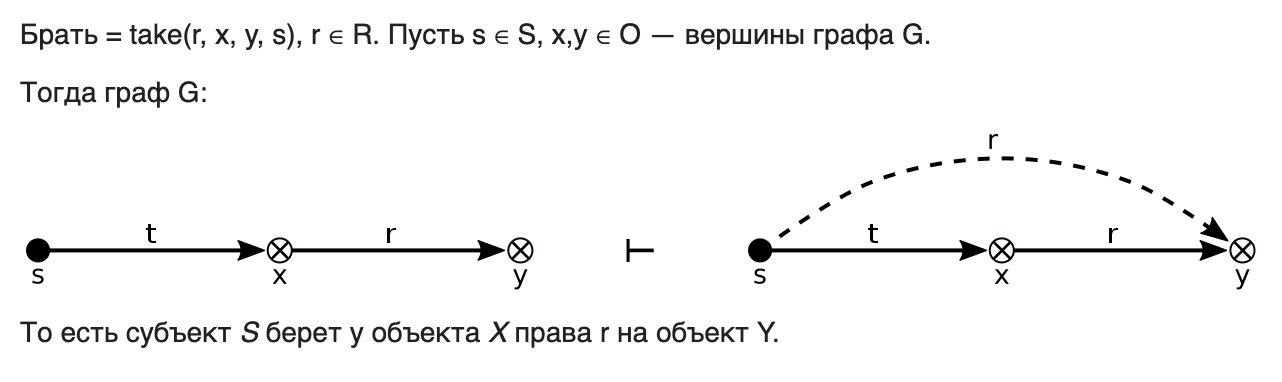
\includegraphics[width=0.8\textwidth]{assets/models/take_grant_bring.png}
\end{figure}

\textbf{Правило «давать».}
\begin{figure}[H]
    \centering
    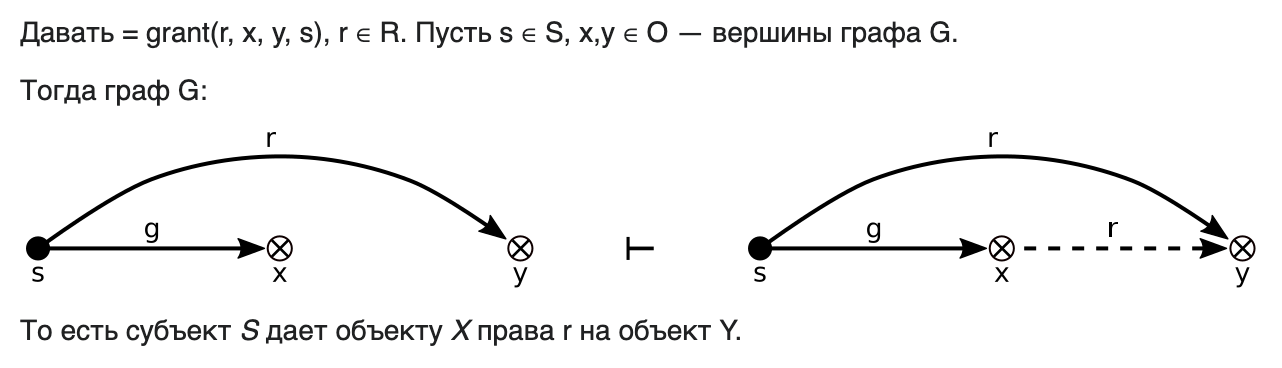
\includegraphics[width=0.8\textwidth]{assets/models/take_grant_give.png}
\end{figure}

\textbf{Правило «создать».}
\begin{figure}[H]
    \centering
    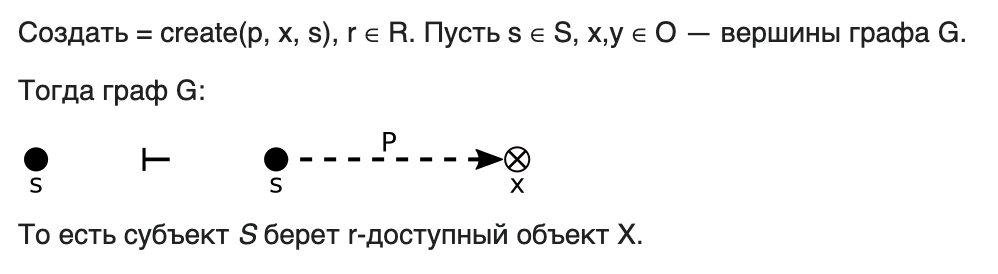
\includegraphics[width=0.8\textwidth]{assets/models/take_grant_create.png}
\end{figure}

\textbf{Правило «удалить».}
\begin{figure}[H]
    \centering
    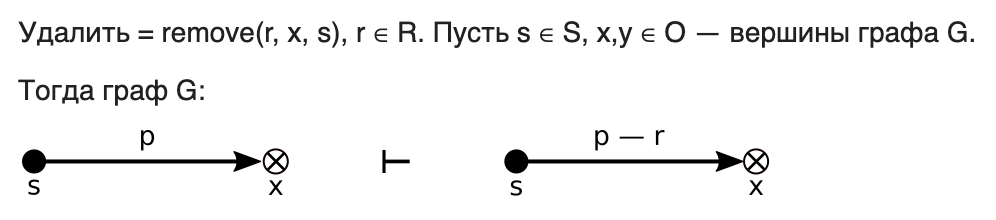
\includegraphics[width=0.8\textwidth]{assets/models/take_grant_delete.png}
\end{figure}

По-сути критерием безопасности системы при использовании модели Take-Grant является невозможность нарушения 
прав доступа при выполнении установленных правил.

Результатом модели становится представление системы как направленного графа с дугами - правами между субъектами 
и объектами.

Следующие две модели намного менее популярны, поэтому при их рассмотрении ссылаемся только на англоязычные 
источники.

\paragraph{Action-Entity}

Модель Acten (Action Entity) была предложена Буссолати и др. \autocite{Jalili} в 1983 г. Является расширением 
модели Take-Grant \autocite{SecModels}:
\begin{itemize}
    \item Дополнительные административные привилегии (использование, создание, удаление, ...)
    \item Предикаты авторизации -- условия, которые должны быть выполнены для предоставления доступа
    \item Представление с использованием двух графиков (один для авторизации для статических действий и один 
    для авторизации для динамических действий)
\end{itemize}
Цели расширения \autocite{Jalili}:
\begin{itemize}
    \item Исправление неизбирательности админских привилегий
    \item Увеличение контроля над транспортным потоком
\end{itemize}

\textit{Каждый элемент системы, имеющий отношение к безопасности, рассматривается как \textbf{сущность (Entity)} \autocite{Jalili}}:
\begin{itemize}
    \item Сущность касается как субъектов, так и объектов
    \item Сущности -- это типы ресурсов
\end{itemize}

\textit{Выделяют два режима доступа -- \textbf{действия (Action)} \autocite{Jalili}}:
\begin{itemize}
    \item cтатический;
    \item динамический.
\end{itemize}

\textbf{Статические действия (режим доступа).} Их выполнение не изменяет аутентификацию и состояние системы.
Состоят из \autocite{SecModels}:
\begin{itemize}
    \item «Использование»: между пользователями, операторами и ресурсами ввода-вывода, приложениями, ...
    \item «Чтение»: для доступа к содержимому объекта
    \item «Написание» («Обновление»)
    \item «Создание»: сущностей
    \item «Удаление»: объекта
\end{itemize}

\textbf{Динамические действия (режим доступа).} Их выполнение изменяет аутентификацию и/или состояние системы.
Состоят из \autocite{SecModels}:
\begin{itemize}
    \item «Грант» (предоставить, Grant): удержание субъектом Ei статического режима m по отношению к Ek 
    позволяет Ei предоставить субъекту Ej режим m на Ek
    \item «Отозвать»
    \item «Делегировать»: позволяет Ei предоставлять Ej динамическое разрешение на «грант», относящееся к режиму m 
    на Ek. Авторизация для делегирования/отмены ограничена несколькими объектами
    \item «Отменить»
\end{itemize}

Вводится иерархия отношений между статическими режимами \autocite{Jalili}:
\begin{itemize}
    \item «Создание»/«Удаление» -- 4
    \item «Обновление» -- 3
    \item «Чтение» -- 2
    \item «Использование» -- 1
\end{itemize}

И между динамическими режимами (административными правами) \autocite{Jalili}:
\begin{itemize}
    \item «Делегировать»/«Отменить» -- 2
    \item «Грант»/«Отозвать» -- 1
\end{itemize}

В соответствии с этими иерархиями в модели Action Entity строят два графа:
\begin{itemize}
    \item cтатических режимов;
    \item динамических режимов.
\end{itemize}

Вводят определённые правила для двух графов, которые являются критерием безопасности системы \autocite{SecModels}.
Подробное изложение можно найти в \autocite{SecModels} и в \autocite{Jalili}.

\paragraph{Wood}

Единственным источником, где удалось найти хоть какую-то информацию о модели Woods является \autocite{Jalili}. 
Согласно нему модель была разработана в 1979 г. Вудсом. Ориентация модели на управлении аутентификацией и контролем 
доступа в БД многоуровневой схемы. Модель рассматривает трехуровневую модель ANSI / SPARC, включая:
\begin{itemize}
    \item Внешний уровень: ближайший к пользователю
    \item Концептуальный уровень: представление данных
    \item Внутренний уровень: ближайший к физическому хранению, не привязанный к аппаратным элементам.
\end{itemize}

Субъекты -- пользователи системы:
\begin{itemize}
    \item Авторизатор, который управляет авторизацией
    \item Пользователи, имеющие доступ к данным
\end{itemize}

Объекты -- объекты концептуального уровня: каждый O принадлежит к категории типа, заданной функцией n(O), 
указывает свою категорию типа (n (O)):
\begin{itemize}
    \item Категории типов на концептуальном уровне: набор сущностей, тип отношения и атрибут
    \item Атрибут может быть связан с одним набором объектов и сопоставляет набор объектов с набором значений
    \item Тип отношения -- это двунаправленная ассоциация между двумя наборами сущностей и может иметь два имени
\end{itemize}

Cостояние авторизации указывается в правилах доступа. Правила доступа имеют вид <s, o, t, p>, где субъект s 
реализует режим доступа t к объекту o при условии p. Правила доступа определяются авторизатором. Основные правила 
указаны в концептуальном уровне, который представляет собой глобальное представление данных организации. Определение 
таблицы (на внешнем уровне) включает ограничения доступа, определяющие, какие типы доступа допустимы для
каждый внешний объект e (каждая таблица и ее поля). Эти ограничения хранятся в ограничении доступа (Access Constraint, AC).

\subsubsection{Мандатные модели}

Основным пунктом каждой мандатной модели безопасности (доступа) является \textbf{определение порядка установления 
мандатных связей} -- задают связи между уровнями доступа и уровнями безопасности (секретности). Каждая модель 
должна ссылаться на доказательство соответствующей теоремы о том, что система, находящаяся в безопасном 
состоянии, не может перейти в небезопасное состояние при соблюдении всех установленных правил и ограничений.

Кратко рассмотрим основные (наиболее популярные) модели безопасности.

\paragraph{Bell-LaPadula}

Мандатный принцип построения системы разграничения доступа в СУБД реализует многоуровневую модель безопасности 
данных \autocite{Skakun}, называемую еще моделью Белл-ЛаПадула (по имени ее авторов - Д. Белла и Л. ЛаПадула), 
введенную в 1975 г.

В многоуровневой модели задается порядок следования уровней доступа и уровней безопасности (секретности), 
а затем устанавливаются связи между уровнем доступа и уровнем секретности - мандатные связи.

Контроль доступа осуществляется в зависимости от уровней безопасности взаимодействующих сторон на 
основании двух правил \autocite{URFULecture10Models}:
\begin{enumerate}
    \item \textbf{No read up (NRU)} – нет чтения вверх: субъект имеет право читать только те документы, 
    уровень безопасности которых не превышает его собственный уровень безопасности

    \item \textbf{No write down (NWD)} – нет записи вниз: субъект имеет право заносить информацию только 
    в те документы, уровень безопасности которых не ниже его собственного уровня безопасности
\end{enumerate}

\textit{Первое правило обеспечивает защиту информации, обрабатываемой более доверенными 
(высокоуровневыми) лицами, от доступа со стороны менее доверенных (низкоуровневых). Второе правило 
предотвращает утечку информации (сознательную или несознательную) от высокоуровневых участников 
процесса обработки информации к низкоуровневым.}

\paragraph{Biba}

Модель Биба или Модель целостности Биба, разработанная Кеннетом Дж. Бибой в 1975 году, представляет собой 
формальную систему перехода между состояниями политики компьютерной безопасности, которая описывает набор 
правил контроля доступа, предназначенных для обеспечения целостности данных. Данные и субъекты сгруппированы 
по упорядоченным уровням целостности. Модель разработана таким образом, чтобы субъекты не могли повредить 
данные на уровне выше, чем субъект, или быть искаженными данными с более низкого уровня, чем субъект. В целом 
модель была разработана для рассмотрения целостности как основного принципа, который является прямой 
противоположностью модели Белл–ЛаПадула \autocite{Biba}.

В целом сохранение целостности данных преследует три цели:
\begin{enumerate}
    \item Предотвратить изменение данных неавторизованными сторонами
    \item Предотвращение несанкционированного изменения данных уполномоченными лицами
    \item Поддерживать внутреннюю и внешнюю согласованность (т.е. данные отражают реальный мир)
\end{enumerate}

Модель Биба определяет набор правил безопасности, первые два из которых аналогичны, но противоположны 
правилам Белл–ЛаПадулы \autocite{Biba}:
\begin{enumerate}
    \item Свойство простой целостности утверждает, что субъект с заданным уровнем целостности не должен читать 
    данные с более низким уровнем целостности (без чтения)
    \item Свойство целостности * (звездочка) указывает, что субъект с заданным уровнем целостности не должен 
    записывать данные с более высоким уровнем целостности (без записи)
    \item Свойство вызова указывает, что процесс снизу не может запрашивать более высокий доступ; только с 
    предметами равного или более низкого уровня
\end{enumerate}

\paragraph{Dion}

(1981) Предлагается в качестве обязательной политики, которая одновременно обеспечивает секретность и целостность. 
Сочетает в себе принципы модели Biba (политика строгой последовательности). В модели нет дискреционной 
политики. Не позволяет передавать информацию от объектов к субъектам (через операции записи). Поток данных 
разрешен только между объектами, но никогда между объектами и субъектами. Содержит введение концепции связи между 
объектами для обмена информацией между ними \autocite{Jalili2}.

Субъекты -- это сущности, выполняемые в системе от имени пользователей. Каждому системному объекту назначается 
3 уровня безопасности и 3 уровня целостности \autocite{Jalili2}:
\begin{itemize}
    \item ASL (Absolute Security Level) указывается при создании и фиксируется на всю жизнь предмета. Это второй уровень 
    пользователя, соответствующий теме
    \item RSL (Read Security Level) -- это самый высокий уровень безопасности, с которого субъекту разрешено читать
    \item WSL -- это самый низкий уровень безопасности, на который субъекту разрешено писать
    \item AIL (Absolute Integrity Level) присваивается при создании и фиксируется на всю жизнь субъекта. Это уровень 
    целостности пользователя, соответствующий предмету
    \item RIL: самый низкий уровень целостности, с которого субъекту разрешено читать
    \item WIL: наивысший уровень целостности, на который субъекту разрешено писать.
\end{itemize}

Устанавливаются ограничения -- для каждого субъекта s \autocite{Jalili2}:
\begin{figure}[H]
    \centering
    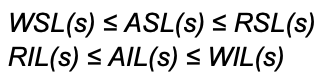
\includegraphics[width=0.8\textwidth]{assets/models/dion_subjects.png}
\end{figure}

Субъект для которого строго соблюдается хотя бы одно неравенство удовлетворенный считается доверенным. Субъект может 
быть доверенным с точки зрения секретности, целостности или того и другого. Субъекты, для которых 4 отношения 
удовлетворяются знаком равенства, считаются недоверенными \autocite{Jalili2}.

Объекты -- любая сущность хранения данных в системе. Каждому объекту назначается 3 уровня безопасности и 
3 уровня целостности \autocite{Jalili2}:
\begin{itemize}
    \item ASL (Absolute sec level) -- уровень безопасности данных, содержащихся в объекте; фиксируется на весь срок 
    службы объекта
    \item MSL (Migration sec level) -- это самый высокий уровень безопасности, на который могут передаваться данные 
    в объекте
    \item CSL (Corruption sec level) - это самый низкий уровень безопасности, с которого данные могут поступать в объект
    \item AIL (Absolute int level) - это уровень целостности данных в объекте
    \item MIL (Migration int level) - это самый низкий уровень целостности, на который могут передаваться данные в объекте
    \item CIL (Corruption int level) - это самый высокий уровень целостности, с которого данные могут поступать в объект
\end{itemize}

Аналогично \autocite{Jalili2}:
\begin{figure}[H]
    \centering
    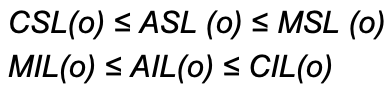
\includegraphics[width=0.8\textwidth]{assets/models/dion_objects.png}
\end{figure}

В модели вводится ряд дополнительных аксиом и правил на отношения между субъектами и объектами.

\paragraph{SeaView}

Модель SEcure dAta VIEW была предложена Дороти Деннингом в 1987 г. Её целью стала защита систем реляционных БД 
\autocite{Jalili2}.

В модели безопасных представлений данных (SeaView) уровни безопасности назначаются каждому элементу данных в 
атрибутах кортежей в отношении. В модели SeaView данные хранятся в наборе одноуровневых фрагментов, а 
многоуровневые отношения реализованы как представления по этим одноуровневым отношениям \autocite{Osama}.

Есть два алгоритма, которые используются при реализации модели SeaView \autocite{Osama}:
\begin{enumerate}
    \item Алгоритм декомпозиции разбивает многоуровневое отношение на одноуровневые фрагменты
    \item Алгоритм восстановления восстанавливает исходное многоуровневое отношение из фрагментов
\end{enumerate}

В модели SeaView декомпозиция многоуровневых отношений на одноуровневые выполняется с применением двух разных 
типов фрагментации: горизонтальной и вертикальной. Таким образом, многоуровневое отношение будет храниться в 
виде пяти одноуровневых фрагментов (одно отношение группы первичного ключа и четыре отношения группы атрибутов).

Модель SeaView имеет много проблем из-за алгоритмов декомпозиции и восстановления. Эти проблемы будут упомянуты 
следующим образом \autocite{Osama}:
\begin{itemize}
    \item Повторные соединения: из-за вертикальной фрагментации, которая используется в модели SeaView, запрос, 
    который включает несколько атрибутов, будет использовать множество повторяющихся левых внешних соединений 
    между несколькими одноуровневыми отношениями для получения результата
    \item Ложные кортежи: когда алгоритм восстановления SeaView применяется к одноуровневым отношениям, 
    дополнительные кортежи будут вставлены в исходное отношение. Эти дополнительные кортежи называются ложными 
    кортежами и являются результатом повторяющихся соединений между одноуровневыми отношениями
    \item Неполнота: алгоритм декомпозиции SeaView накладывает ограничения на возможности базы данных. Некоторые 
    экземпляры отношений, которые имеют реалистичную и полезную интерпретацию в реальной жизни, не могут быть 
    реализованы в модели SeaView
    \item Левое внешнее соединение: алгоритм восстановления SeaView основан на левом внешнем соединении отношений. 
    Хорошо известно, что соединение - это дорогостоящая операция, и ее следует по возможности избегать
\end{itemize}

\paragraph{Jajodia\&Sandhu}

Модель Джаджодиа–Сандху является производной от модели SeaView. Она модифицирует алгоритм, который разлагает 
многоуровневое отношение на одноуровневые фрагменты, а также модифицирует алгоритм восстановления, который 
восстанавливает исходное многоуровневое отношение \autocite{Osama}.

В модели Джаджодиа–Сандху алгоритм декомпозиции использует только горизонтальную фрагментацию, поскольку 
вертикальной фрагментации не требуется. Это приводит к улучшению алгоритма восстановления в модели Джаджодиа–Сандху 
по сравнению с алгоритмом восстановления в модели SeaView, поскольку можно восстановить многоуровневое отношение 
без необходимости выполнять операции соединения; для восстановления многоуровневого отношения требуются только 
операции объединения \autocite{Osama}.

В модели Джаджодиа–Сандху есть две основные проблемы \autocite{Osama}:
\begin{itemize}
    \item Семантическая неоднозначность: предположим, что есть два кортежа в отношениях с уровнями безопасности 
    U и S, и нет кортежа с уровнем безопасности TS. Если пользователю с уровнем безопасности TS необходимо 
    получить информацию из отношения, он не может решить, какая информация является правильной, потому что 
    значения из кортежа U и кортежа S в отношении будут извлечены в результате запроса
    \item Операционная неполнота: предположим, что существует два несравнимых уровня безопасности, M1 и M2, 
    наименьшая верхняя граница которых соответствует уровню безопасности S, а наибольшая нижняя граница -- 
    уровню безопасности U. Пользователь с уровнем безопасности S не может вставлять кортежи, которые содержат 
    атрибуты с уровнями безопасности U, M1 и M2
\end{itemize}

\paragraph{Smith\&Winslett}

В модели Смита–Уинслетта многоуровневая реляционная база данных рассматривается как набор обычных реляционных 
баз данных, в которых все базы данных используют одну и ту же схему. Эта модель не поддерживает безопасность 
на уровне каждого отдельного атрибута. Уровень безопасности может быть назначен только атрибутам первичного 
ключа и кортежам в целом \autocite{Osama}.

Многоуровневая реляционная схема задается как R(A\textunderscore{pk}, C\textunderscore{pk}, A\textunderscore{{1} 
..., A\textunderscore{n}, TC), где A\textunderscore{pk} обозначается как атрибут данных первичного ключа, 
C\textunderscore{pk} - атрибут классификации первичного ключа, который содержит уровень безопасности первичного 
ключа. Атрибут данных A\textunderscore{1} ... A\textunderscore{n} обозначается как атрибуты данных, а TC 
обозначается как атрибут классификации кортежа, который содержит уровень безопасности кортежа \autocite{Osama}.

Согласно этим правилам определяется доступ для обновления и чтения. Модификация базы данных (вставка, удаление 
и обновление) пользователем может изменить данные только на уровне безопасности пользователя. Запрос от пользователя 
с уровнем безопасности L может получить доступ к данным именно из тех баз данных, уровень которых не выше уровня L 
\autocite{Osama}.

В этой модели была добавлена семантика, основанная на концепции веры. Модель Смита–Уинслетта также известна как 
модель семантики, основанная на убеждениях, а также представила концепцию базового кортежа. Базовый кортеж -- 
это самый низкий уровень безопасности кортежа базы данных, в котором утверждается существование объекта. 
Таким образом, процедура обновления устраняет проблемы, присутствующие в модели Джаджодиа–Сандху, но ограничивает 
объем обновления одним объектом \autocite{Osama}.

\paragraph{Решеточная}

Управление доступом на основе решеток (Lattice-Based Access Control, LBAC) - это сложная модель управления доступом, 
основанная на взаимодействии между любой комбинацией объектов (например, ресурсов, компьютеров и приложений) и 
субъектов (таких как отдельные лица, группы или организации) \autocite{LBAC}.

В этом типе модели управления принудительным доступом на основе меток решетка используется для определения уровней 
безопасности, которые может иметь объект и к которым субъект может иметь доступ. Субъекту разрешен доступ к объекту 
только в том случае, если уровень безопасности субъекта больше или равен уровню безопасности объекта \autocite{LBAC}.

Математически уровень безопасности доступа также может быть выражен в терминах решетки (набор частичного порядка), 
где каждый объект и субъект имеют наибольшую нижнюю границу (совпадение) и наименьшую верхнюю границу (соединение) 
прав доступа. Например, если двум субъектам A и B требуется доступ к объекту, уровень безопасности определяется как 
соответствие уровней A и B. В другом примере, если два объекта X и Y объединены, они образуют другой объект Z, 
которому присваивается уровень безопасности, образованный объединением уровней X и Y \autocite{LBAC}.

LBAC также известен как ограничение управления доступом на основе меток (или управление доступом на основе правил) 
в отличие от управления доступом на основе ролей (RBAC) \autocite{LBAC}.

Модели управления доступом на основе решетки были впервые формально определены Деннингом (1976).

\subsubsection{БД с многоуровневой секретностью (MLS)}
\subsubsection{Многозначность (областей применения разных моделей)}